\documentclass[letterpaper,10pt,conference]{IEEEtran}
\IEEEoverridecommandlockouts
\usepackage{amsmath}
\usepackage{fullpage}
\usepackage{enumerate}
\usepackage{graphicx}
\usepackage{cite}
\usepackage{subfig}
%\usepackage{natbib}

\title{Kalman Filtering for Improved Fiducial Marker Tracking}
\author{Joe Degol, Jason Rock, Kevin Shih}

\begin{document}
\maketitle
\thispagestyle{empty}
\pagestyle{empty}



%----- Abstract -----%
\begin{abstract}
In this paper, we address some common challenges of current state-of-the-art fiducial marker systems. In particular, we formulate and apply an extended kalman filter for improving detection rates on blurred images, intermittent drops, steep out-of-plane rotations, and significant depths. We provide quantitative results demonstrating the effectiveness of our algorithm for ``hole filling'', and also demonstrate how our system can save on bandwidth by sampling fewer frames. We also provide qualitative results in the form of video sequences.
\end{abstract}
%----- Abstract -----%



%----- Introduction -----%
\section{Introduction}
Fiducial markers are artificial objects added to a scene that can be easily detected. They can take many forms such as planar tags and infrared spheres and have shown utility for applications in motion capture systems, augmented reality \cite{Fiala2005}\cite{Fiala2010}, and robotics \cite{Olson2011}. Figure \ref{fig:applications} depicts some real world applications of fiducial markers.

\begin{figure}
\centering
\includegraphics[scale=.25]{MarkerApplications}
\caption{Fiducial Marker Applications: (A) depicts fiducial markers being used in a motion capture system to track human motion, (B) depicts fiducial markers being used with the Nintendo 3DS handheld video game console for augmented reality, and (C) depicts fiducial markers being used for robot swarm localization.}
\label{fig:applications}
\end{figure}

For robotics applications, planar patterns have emerged as the popular fiducial marker design \cite{Sattar2007,Olson2011}. Planar markers are useful for robotics because a plane to plane homography can be estimated, where the homography also defines the 6 degree of freedom pose of the camera relative to the tag \cite{Olson2011}. However, challenges exist for planar markers. In particular, the tag becomes difficult to detect at steep out-of-plane rotations, far depths, quick motions inducing blur, and camera jitter causing intermitently dropped detections. These challenges are depicted in Figure \ref{fig:challenges}.

\begin{figure}
\centering
\includegraphics[scale=.2]{MarkerChallenges}
\caption{Planar Tag Detection Challenges: (A) depicts difficulty with out-of-plane rotations, (B) depicts difficulty with depth, (C) depicts difficulty with blur, (D) depicts difficulty with intermittent detection drops.}
\label{fig:challenges}
\end{figure}

In this project, we investigate how Kalman Filtering can be used to address the aforementioned challenges. Unlike common tracking problems such as face tracking, we require that the tracker tightly follow the four corners of a fiducial marker through various viewpoint changes. The remainder of this paper is presented as follows: Section \ref{sec:approach} outlines our approach, Section \ref{sec:results} presents our results, and Section \ref{sec:conclusion} provides concluding remarks and each group members contributions.
%----- Introduction -----%



%----- Approach -----%
\section{Approach}
\label{sec:approach}
\begin{figure}
\centering
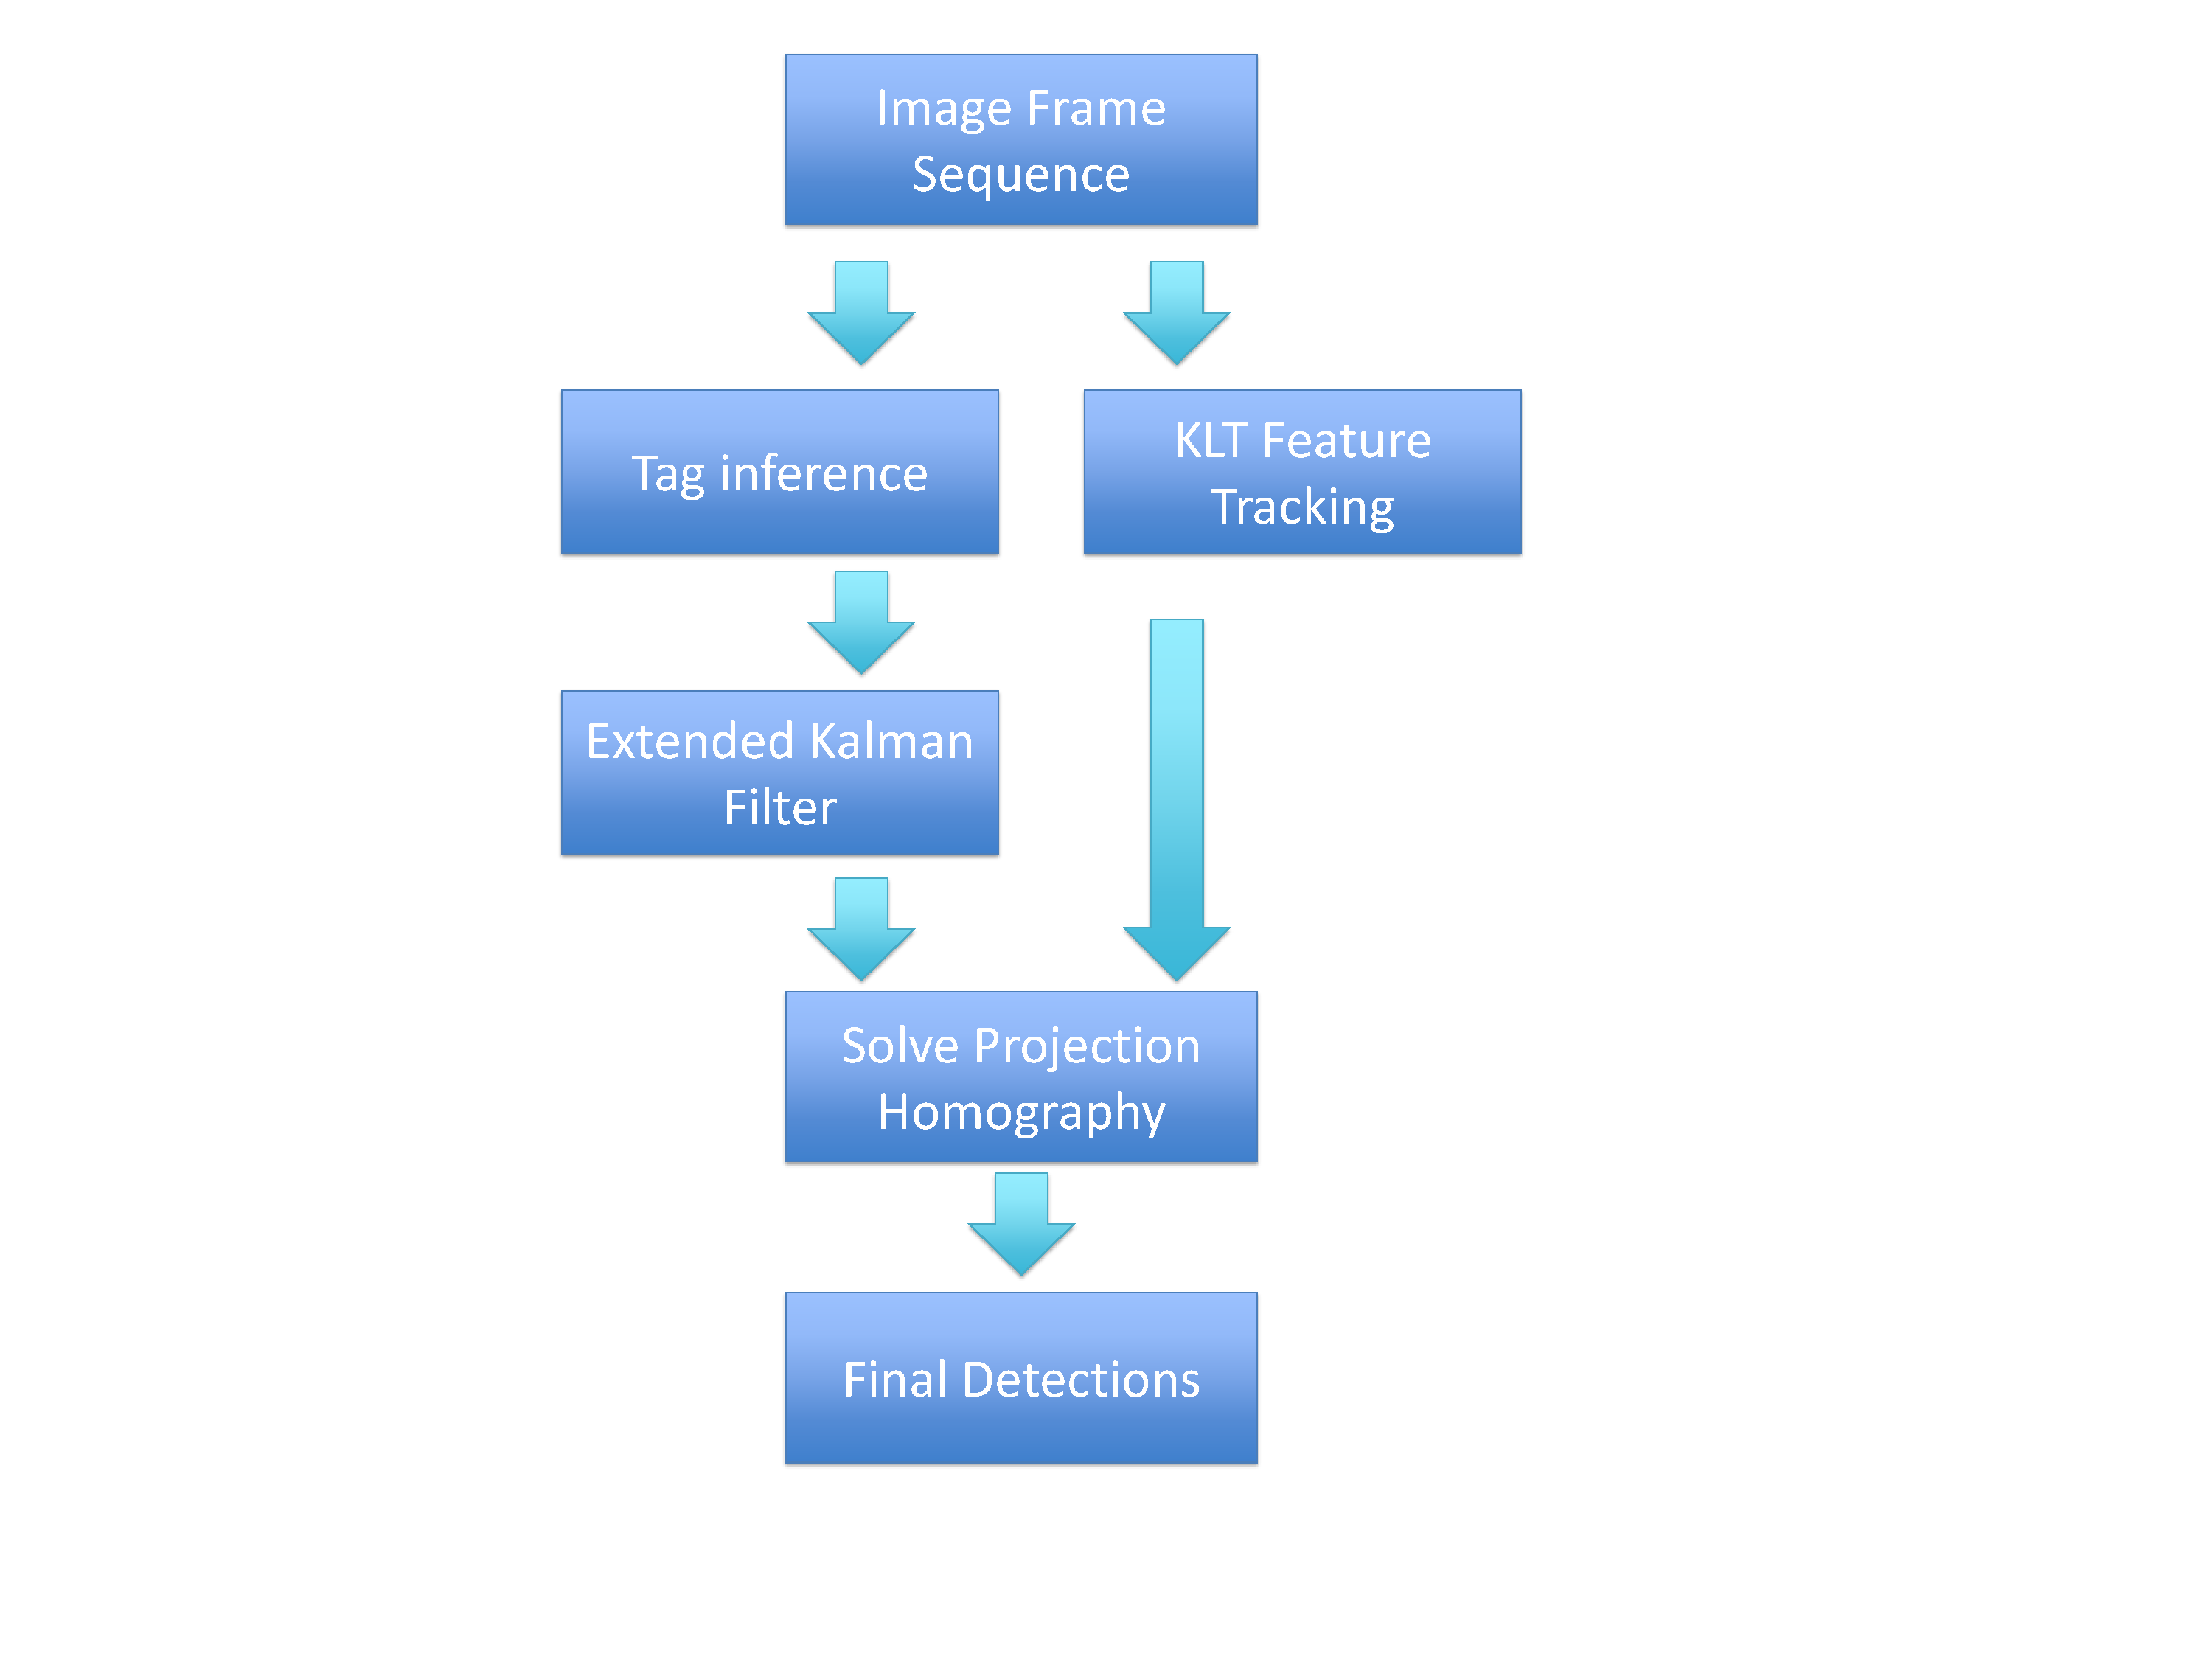
\includegraphics[scale=.15]{flowchart.pdf}
\caption{Flow Diagram of Method: We begin with an image sequence. We then use Tag inference and KLT feature tracking. Extended Kalman filtering is used when tag inference fails to define a bounding region on tag movement. KLT points from within this bounding region are fed to RANSAC for homography estimation. Homography estimation defines the new tag boundary.}
\end{figure}

Because the fiducial marker detection can be efficiently run in real time, we opt to use it when it is available. However, because its parameters are set to cut off at very high precisions to avoid false positives, tag detections are often missed in frames where there is too much motion blur or the size of the tag is too small due to distance or angle.

Our overall approach is as follows:
\begin{enumerate}
\item Extract tag detections using AprilTags fiducial marker detection \cite{Olson2011}
\item Track interest points across image sequences using the KLT Feature Tracker \cite{Lucas1981,Shi1994,Tomasi1991}
\item Smooth over detection gaps with Extended Kalman Filtering(EKF) \cite{Thrun2005}
\item Compute projective transformation on tracked feature points within EKF proposed area \cite{Forsyth2002}
\item Apply projection to bounding quadrilateral from previous frame to determine new 4-corner coordinates
\end{enumerate}

\subsection{Detecting Fiducial Markers}
We used AprilTags \cite{Olson2011} for our choice of fiducial marker. We ran the provided detection code over each frame using default parameters and recorded the 4 corners and center coordinates for each detection.

\subsection{Tracking Interest Points with KLT}
We used the Kanade-Lucas-Tomasi (KLT) Feature Point Tracker \cite{Lucas1981,Tomasi1991,Shi1994} to track feature points in each frame of our video sequence.

\subsection{Kalman Filtering}
Fiducial marker detections are prone to occassional loss and expensive to run for every frame.  It is advantageous to recover from loss and reduce the number of frames which require detection.  This problem lends itself well to an Extended Kalman Filter over the location and size of the fiducial marker.  We use a constant velocity model of the system dynamics, estimating the location and velocity for the three terms.
%\begin{align}
%x_k &= \left[ \begin{array}{cccccc}
%1 & 0 & 0 & d & 0 & 0 \\
%0 & 1 & 0 & 0 & d & 0 \\
%0 & 0 & 1 & 0 & 0 & d \\
%0 & 0 & 0 & 1 & 0 & 0\\
%0 & 0 & 0 & 0 & 1 & 0\\
%0 & 0 & 0 & 0 & 0 & 1
%\end{array}\right] x_{k-1} + w_{k-1}\\
%z_k &= \left[ \begin{array}{cccccc}
%1 & 0 & 0 & 0 & 0 & 0\\
%0 & 1 & 0 & 0 & 0 & 0\\
%0 & 0 & 1 & 0 & 0 & 0\end{array}\right] x_k + v_{k}
%\end{align}

\begin{align}
x_k &= \left[ \begin{array}{cc}
I_{3\times 3} & d\cdot I_{3\times 3}\\
0_{3\times 3} & I_{3\times 3}
\end{array} \right] x_{k-1} + w_{k-1}\\
z_k &= \left[ \begin{array}{cc}
I_{3\times 3} & 0_{3\times 3}
\end{array} \right] x_k + v_k
\end{align}


\subsection{Solving for the Homography}
% cite alumni.media.mit.edu/~cwren/interpolator
The projecton matrix mapping coordinates in frame $t-1$ to frame $t$ has 8 degrees of freedom. Thus, we need at least 4 feature point correspondences from the approximate region of the fiducial tag to solve. 
\begin{equation}
\begin{bmatrix}
x_{t}W\\
y_{t}W\\
W
\end{bmatrix}
= \begin{bmatrix}
a&b&c\\
d&d&f\\
g&h&1\\
\end{bmatrix}
\begin{bmatrix}
x_{t-1}\\
y_{t-1}\\
1
\end{bmatrix}
\end{equation}

Using the proposed region from the Kalman filter, we isolate 4 KLT interest point correspondences using Random Sample Consensus (RANSAC), and output a Homography matrix. If the search area is too small to contain enough points, we slowly expand the radius until enough tracked interest points are available.

\begin{equation}
A(N) = 
\begin{bmatrix}
x_{t-1,N}& y_{t-1,N}&1&0&0&0& -x_{t,N}\\
0&0&0&x_{t-1,N}& y_{t-1,N}&1& -y_{t,N}\\
\end{bmatrix}
\end{equation}

\begin{equation}
B(N) = 
\begin{bmatrix}
-x_{t,N}x_{t-1,N}& -x_{t,N}y_{t-1,N}\\
-y_{t,N}x_{t-1,N} &-y_{t,N}y_{t-1,N}\\
\end{bmatrix}
\end{equation}


\begin{equation}
\begin{bmatrix}
A(1)& B(1)\\
\vdots&\vdots\\
A(N)& B(N) \\
\end{bmatrix}
\begin{bmatrix}
a\\
b\\
c\\
d\\
e\\
f\\
g\\
h\\
\end{bmatrix} = 
\begin{bmatrix}
x_{t,1}\\
y_{t,1}\\
\vdots\\
x_{t,N}\\
x_{t,N}\\
\end{bmatrix}
\end{equation}
%----- Approach -----%



%----- Alternative Methods -----%
\section{Alternative Methods for Orientation Prediction}
\subsection{HMM}
One alternative method we considered was using the HMM in place of the homography. An HMM would be learned using translational distances of the box corners between two frames as observations. These would have to be discretized and coded as a 1 dimensional variable. Its hidden states would be \{UP DOWN LEFT RIGHT\}$\times$\{FORWARD BACKWARD\}. For inference, we would input a given sequence of corner translations (using provided detections) and infer the most likely next state and observations in the sequence.

For this, we collected 24 separate video datasets for each possible hidden state combination. However, we did not finish implementing the HMM for this because we expected it would be too complex and perform worse than our proposed homographic solution.

\subsection{Augmented Kalman Filtering}
Another alternative model that we considered involves estimating location and rotation of the camera using an additional Kalman filter.  However, the parameterization for extrinsics would not have been acceptable as rotation and translation are strongly tied.  We opted for the model described in the approach section, as solving homographies with point correspondences was much simpler and would have worked just as well if not better.
%----- Alternative Methods -----%



%----- Results -----%
\section{Experiments and Results}
\label{sec:results}
We collected six video sequences using a handheld camera moved by a person. Our data was collected in an effort to focus on addressing the challenges previously addressed in Figure \ref{fig:challenges}. Specifically, one dataset (Depth) starts close to the tag and retreats to increase the depth from the tag. Another dataset (OOP Rotation) starts in a forward facing position and moves to steep angles of out-of-plane rotation on both sides of the tag. Two more datasets (Blur Lateral and Blur Depth) begin by moving slowly, then accelerate to produce blurry frames, then slow down again, where the movement occurs in the respective lateral or depth direction. Finally, we have two more datasets (General 1 and 2) that contain aspects of all previous datasets and their respective challenging aspects.

\begin{figure}
\centering
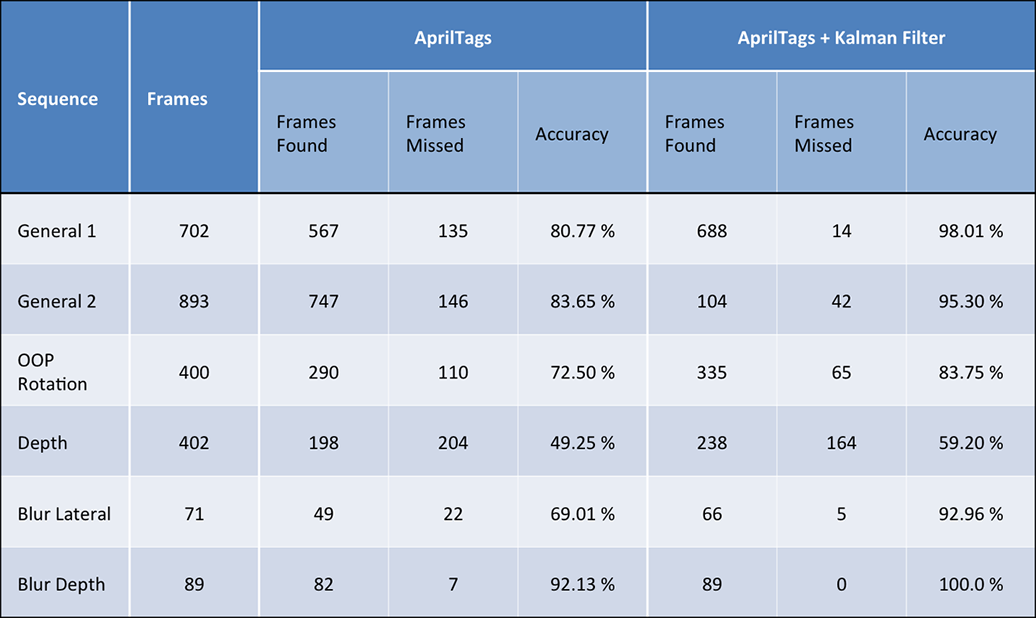
\includegraphics[scale=.4]{table1}
\caption{This table presents results for the baseline and with our system.}
\label{fig:table1}
\end{figure}


We first tested how well the AprilTags system performed on our data sets. The results of this are shown in Figure \ref{fig:table1}. We attribute the lost frames in each sequence to the challenges cases. Next, we included our system with the AprilTags detections. As can be seen, the total number of detections increases with the addition of our system. In Figure \ref{fig:table2}, we present quantitative results addressing which challenges are system works best at rectifying. In particular, Table \ref{fig:table2} shows the number and percent of detections we rectify out of the total missed detections. Based on the results of Figure \ref{fig:table2}, we can see that we rectify over 70\% of the missed detections for General 1, General 2, Lateral Blur, and Depth Blur. This demonstrates that our method works well with Blur and Intermittent drops. We reason that the effectiveness of our method on these cases is because the Kalman Filter is able to accurately estimate the missing regions to perform ``hole filling''. Conversely, our method performs poorly on Depth because once the tag is too far away, it is lost, and the system has no way to update the Kalman Filter with new observations. Thus, the estimate diverges. Similar reasoning can be used to explain our mediocre results with OOP Rotation; however, if the rotation is steep, and then returns to a detectable angle, our system is able to fill that gap.

\begin{figure}
\centering
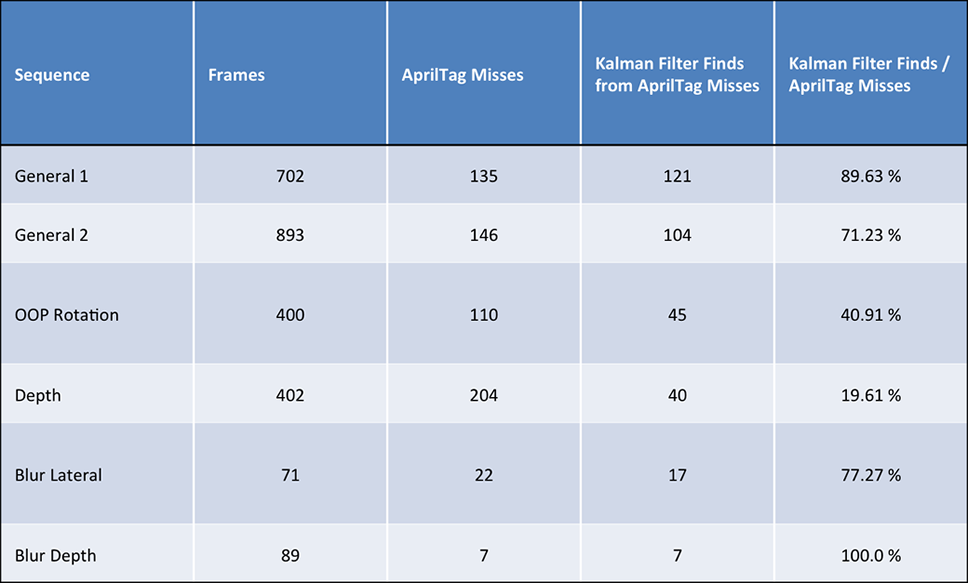
\includegraphics[scale=.4]{table2}
\caption{This table presents our results against each challenge.}
\label{fig:table2}
\end{figure}

Besides hole filling, another practical application of our system would be for degrading the signal intentionally and rely on the kalman filter to fill the gaps. To test this, we sampled the data at a rate between every second to tenth image.  We also sampled randomly such that we had $^1/_2$ to $^1/_{10}$ of the original data.  For the random sample, we performed the sample ten times and averaged the result. We report the error of the Kalman center with the ground truth center.  This error is reported as an average error over all frames for the dataset and is shown in Figure \ref{fig:kalman_error}.

We also evaluate the error of our whole system for estimating the corners of the fiducial marker.  We display results for unsampled data and evenly and randomly sampled data of $^1/_2, ^1/_5, ^1/_10$.  As above, the random sample is the average of ten.  The error reported is the average distance between the predicted corners and the April Tag corners. This error is shown in Figure~\ref{fig:error_plot}
\begin{figure*}
\centering
\subfloat[General 1]{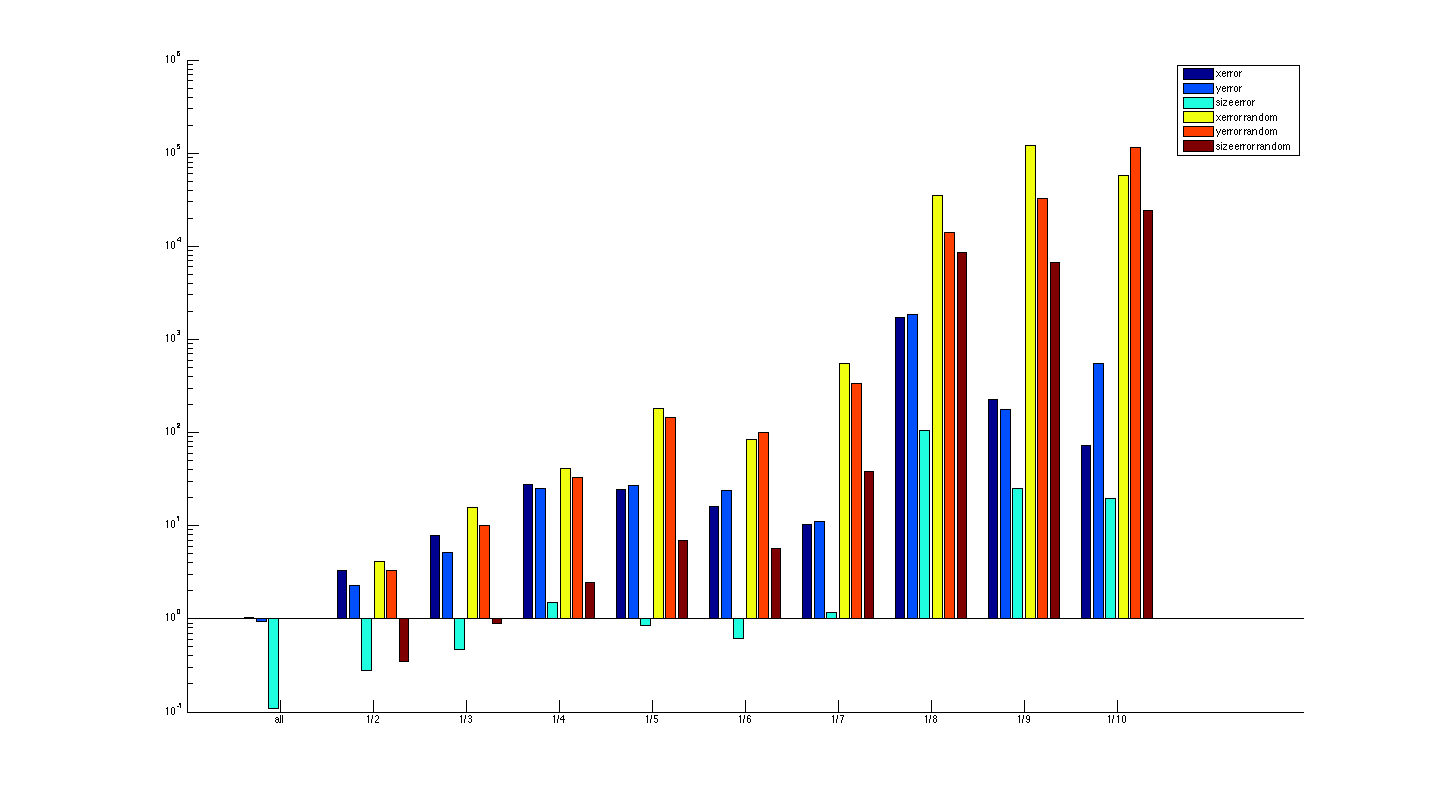
\includegraphics[width=.3\textwidth]{kalman_nov_1}}
\subfloat[Depth]{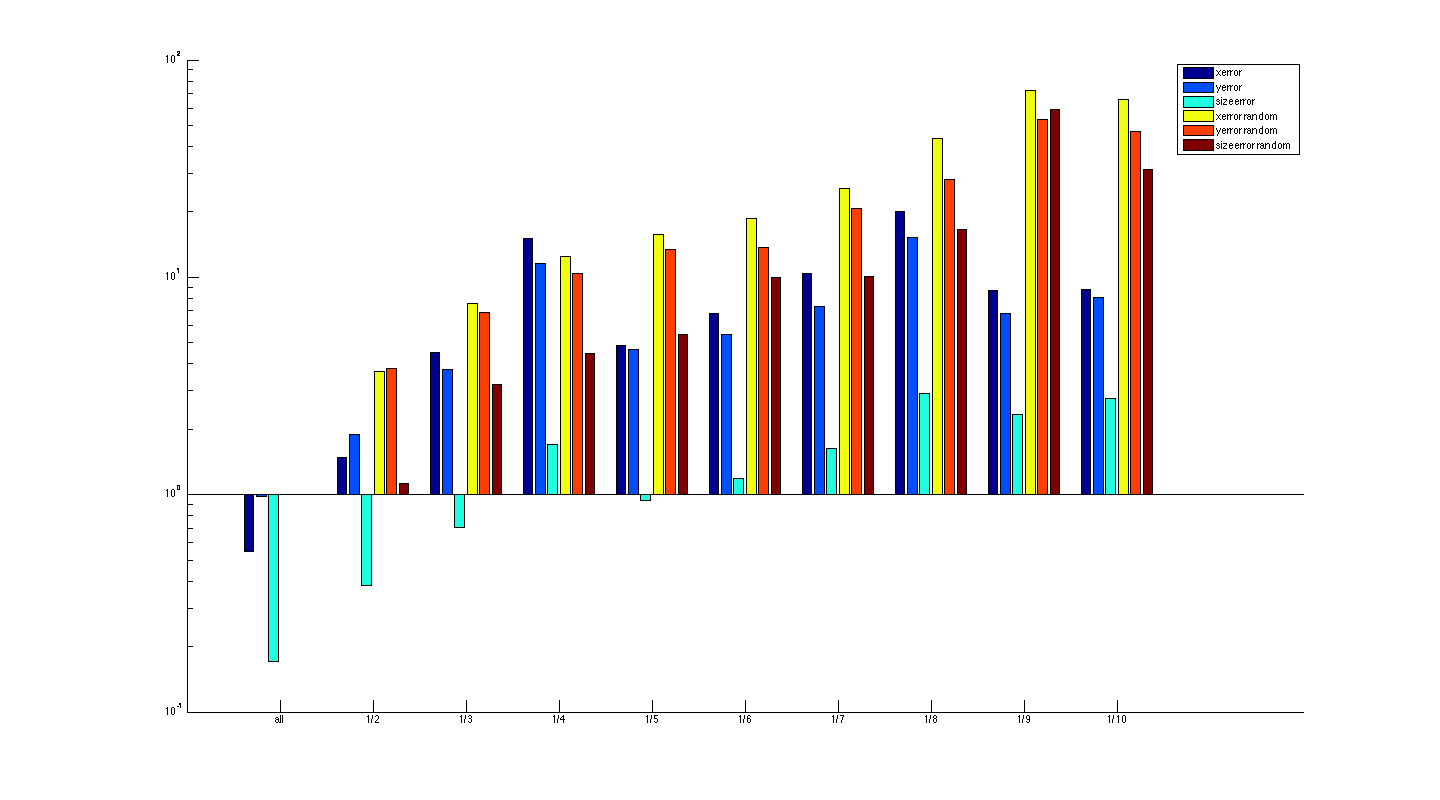
\includegraphics[width=.3\textwidth]{kalman_nov_2}}
\subfloat[Rotation]{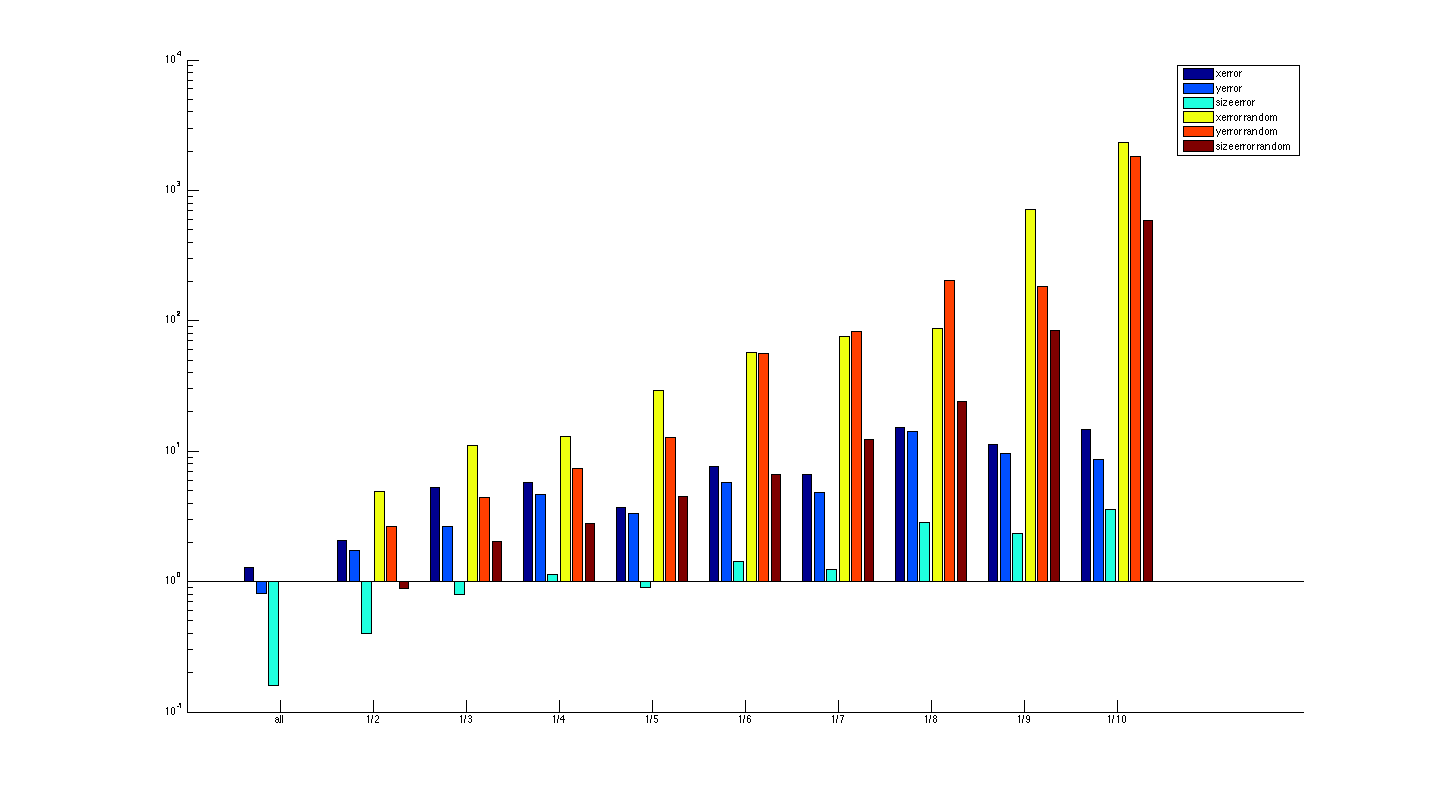
\includegraphics[width=.3\textwidth]{kalman_nov_3}}

\subfloat[General 2]{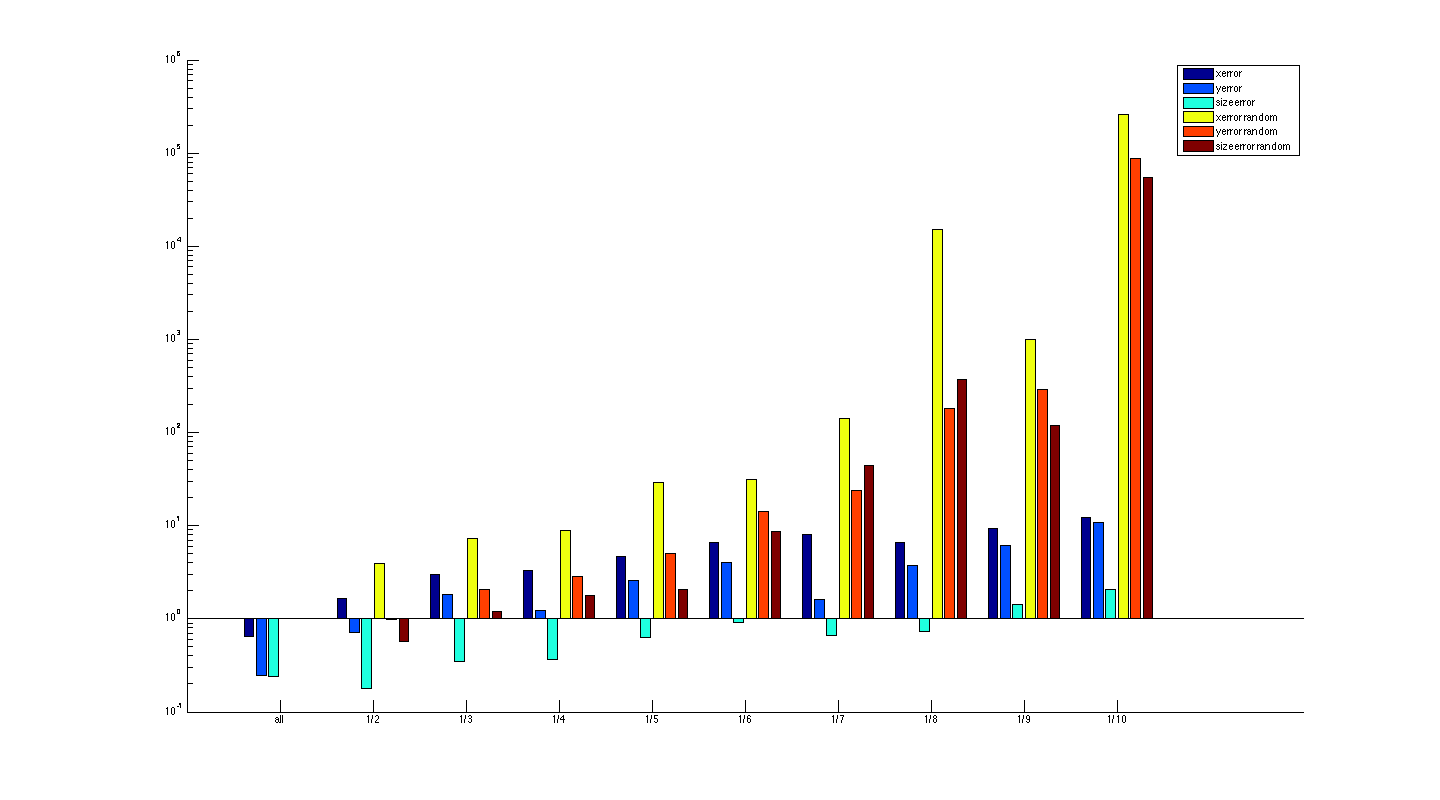
\includegraphics[width=.3\textwidth]{kalman_dec_1}}
\subfloat[Blur Lateral]{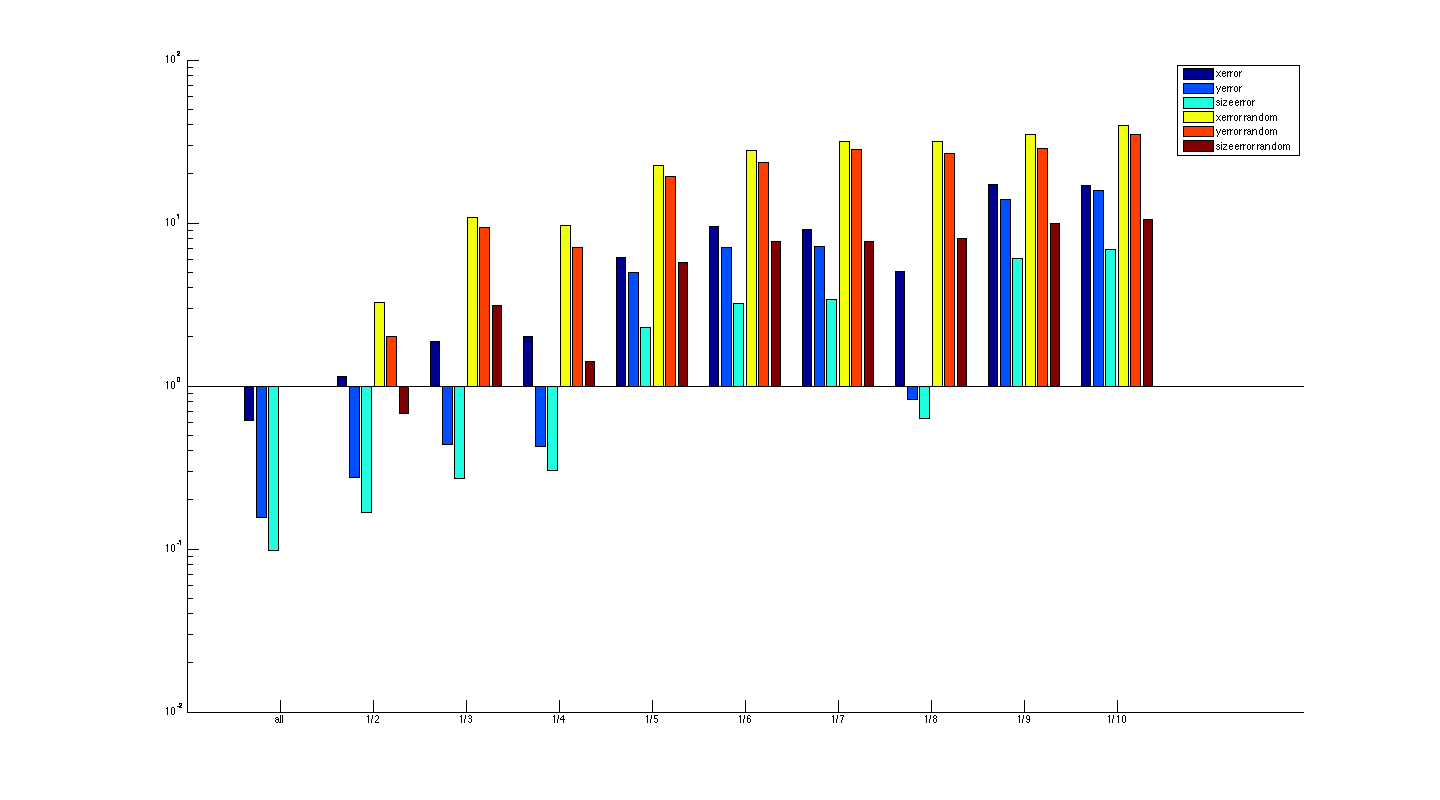
\includegraphics[width=.3\textwidth]{kalman_dec_2}}
\subfloat[Blur Depth]{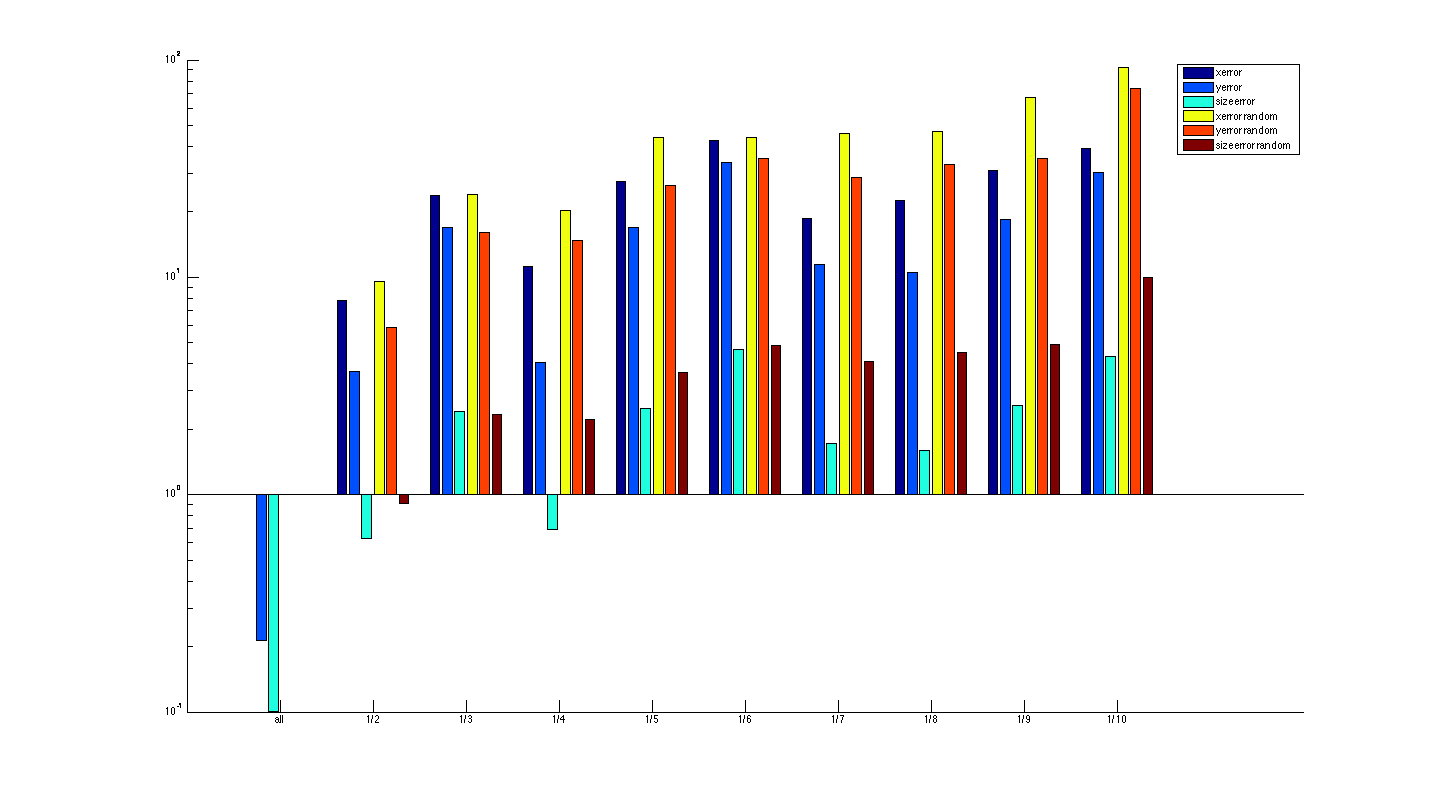
\includegraphics[width=.3\textwidth]{kalman_dec_3}}
\caption{Kalman filter error on all datasets.  It is important to note that the Kalman filter on equally spaced sampling produces results which are often acceptable as compared to random sampling. This implies that systems which evaluate detections at a subset of frames could be designed.}
\label{fig:kalman_error}
\end{figure*}

\begin{figure*}
\centering
\subfloat[General 1]{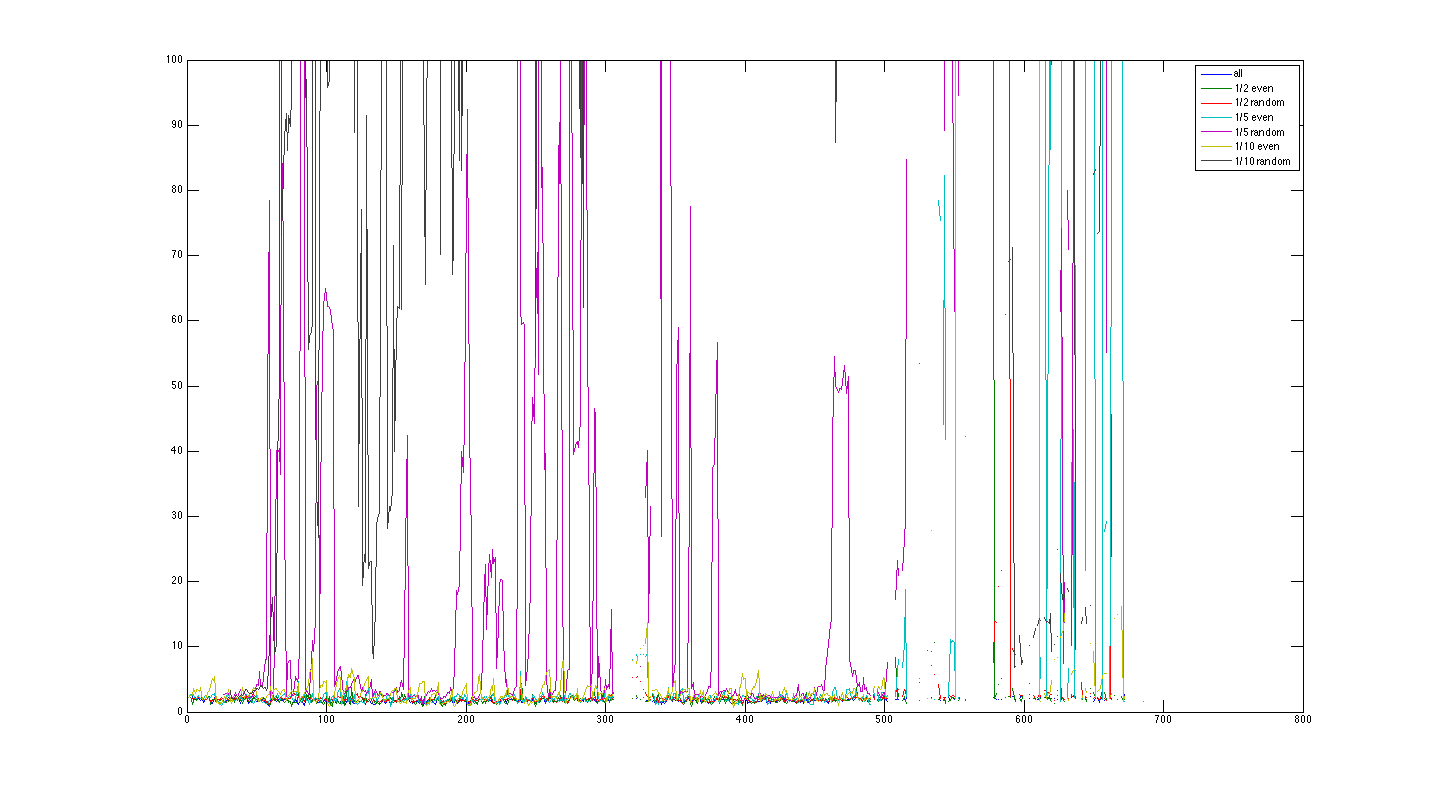
\includegraphics[width=.3\textwidth]{Corner_error_nov1}}
\subfloat[Depth]{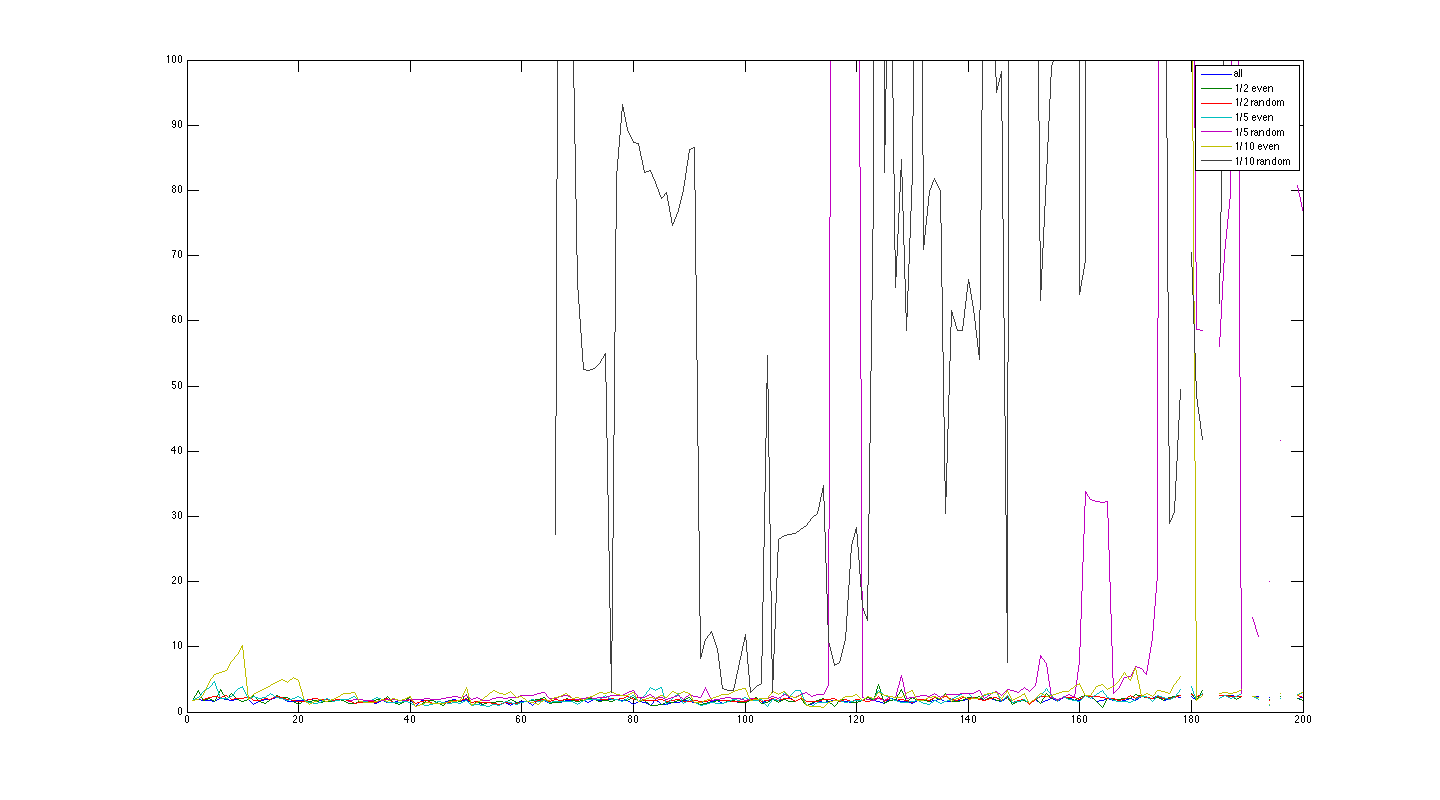
\includegraphics[width=.3\textwidth]{Corner_error_nov2}}
\subfloat[Rotation]{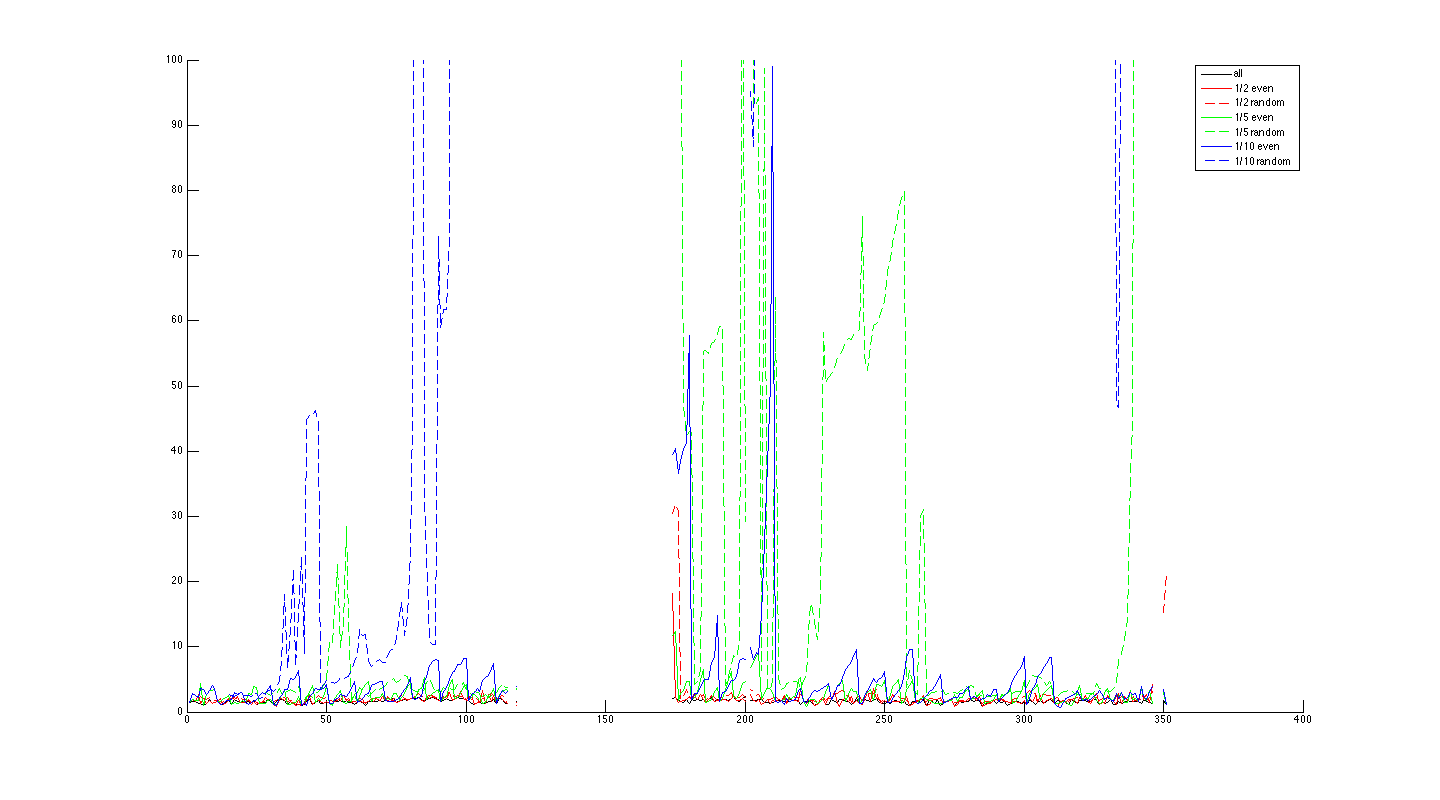
\includegraphics[width=.3\textwidth]{Corner_error_nov3}}

\subfloat[General 2]{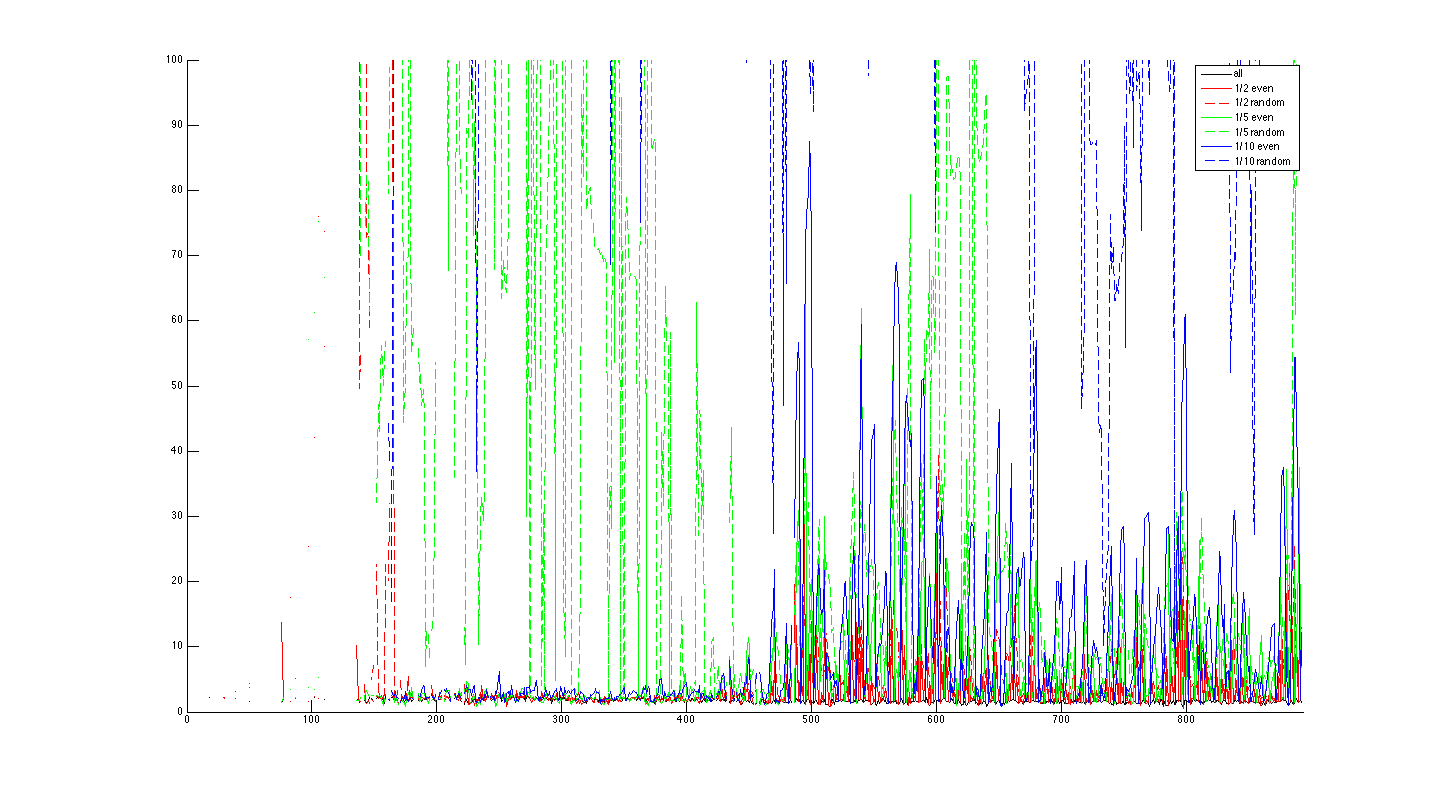
\includegraphics[width=.3\textwidth]{Corner_error_dec1}}
\subfloat[Blur Lateral]{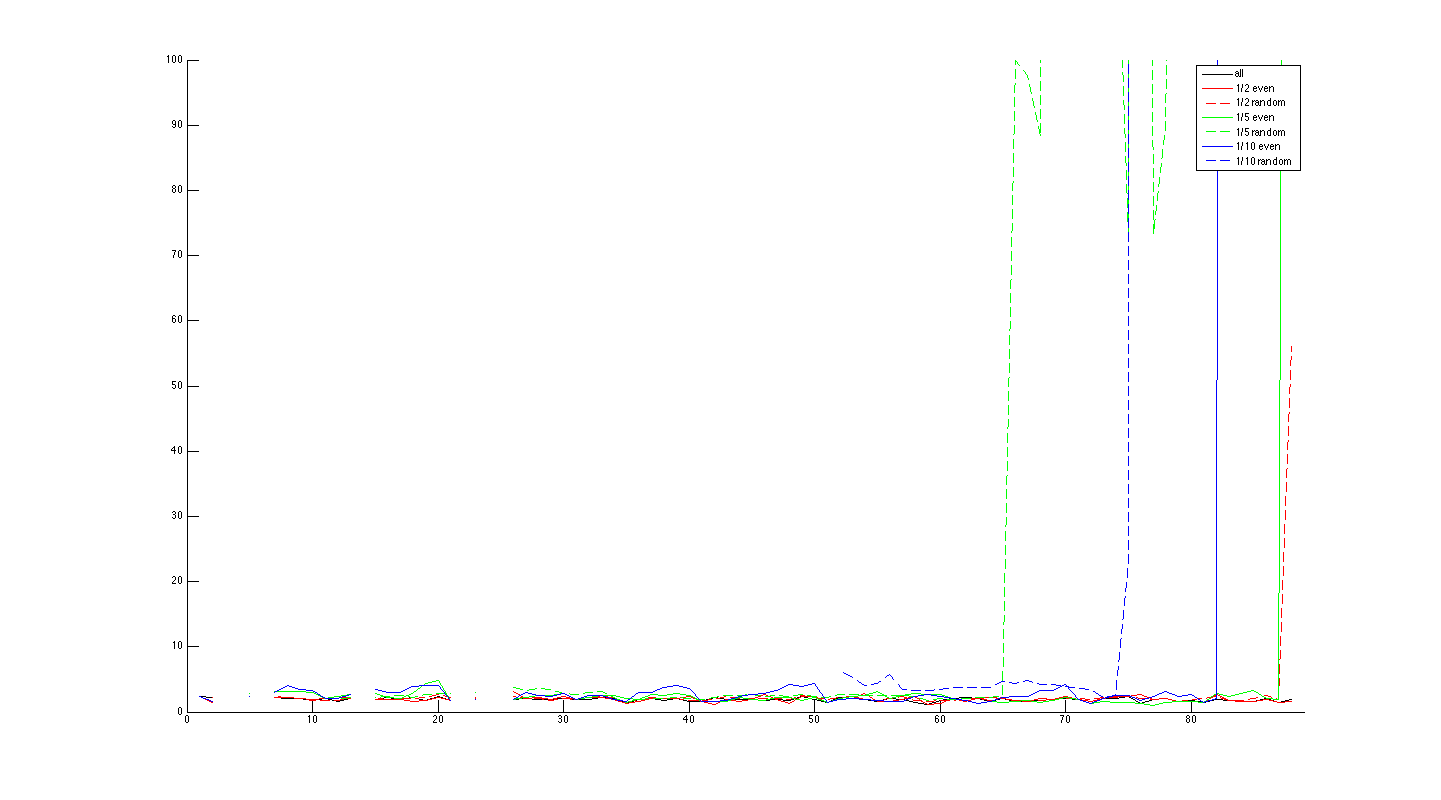
\includegraphics[width=.3\textwidth]{Corner_error_dec2}}
\subfloat[Blur Depth]{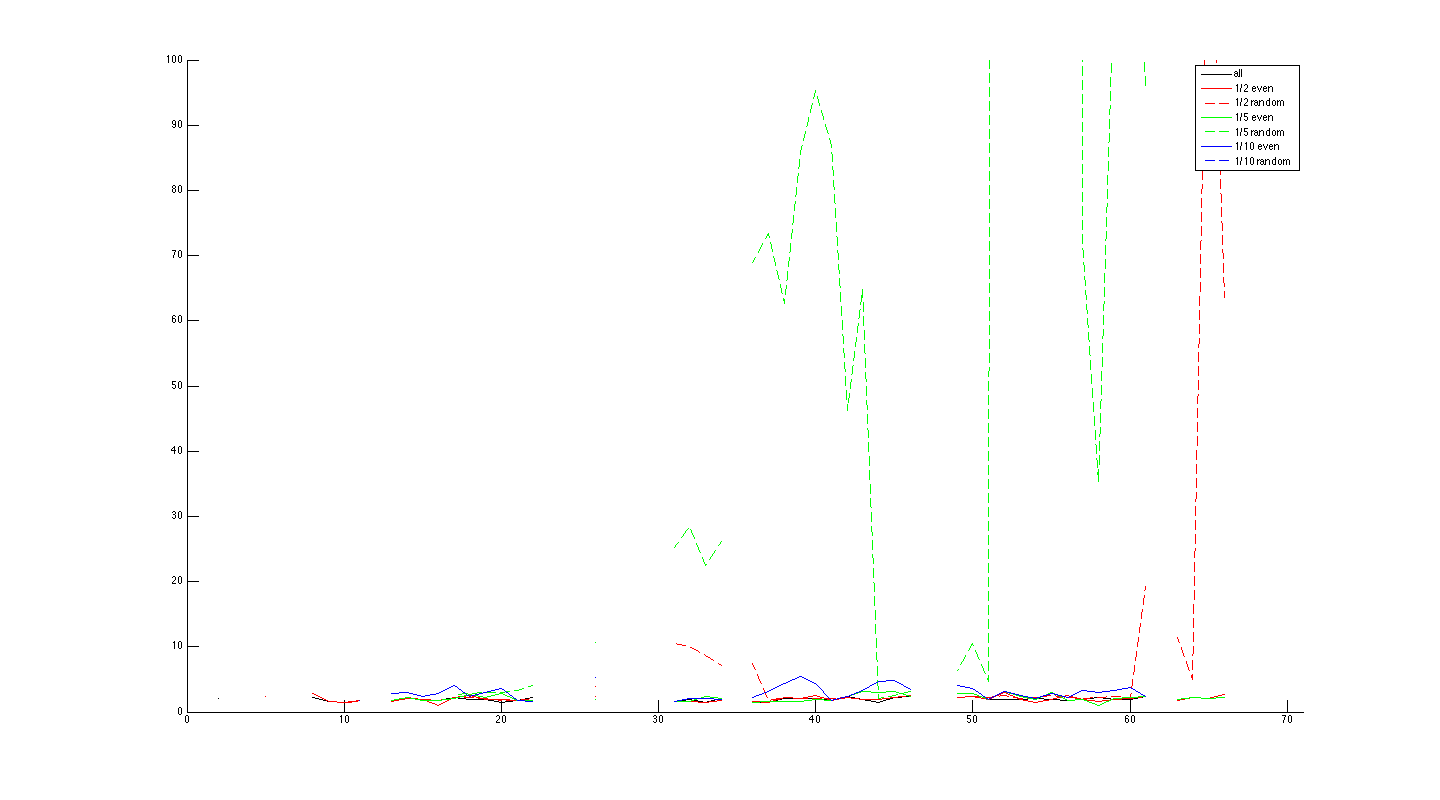
\includegraphics[width=.3\textwidth]{Corner_error_dec3}}
\caption{Average corner error with our system.  The dashed lines represent random sampling, while the solid lines represent even sampling.  Even sampling has a cyclic error as every $k$th frame we reinitialize the tag corners.  For random sampling we see results which are worse due to long runs of no reinitialization.  This causes the Kalman filter to have gross errors.}
\label{fig:error_plot}
\end{figure*}
%----- Results -----%



%----- Conclusion -----%
\section{Conclusion}
\label{sec:conclusion}
In this paper, we present a novel application of the Extended Kalman Filter. We provide a formulation of the Extended Kalman Filter that is appropriate for fiducial marker tracker, and demonstrate that our method is capable of improving current state of the art detections systems by filling in missed detections. We also demonstrate that our method can be used on an intentionally degraded signal. Future work with the project could include employing the pose estimate as part of the estimation; in particular, can filtering be used to smooth the pose estimation while also using the pose estimation to achieve a better estimate on the tag location.

For this project, all authors contributed equally.
\textbf{Joseph DeGol} implemented RANSAC, collected the data, generated the KLT tracks, created the poster and presentation, implemented a ground truthing tool and ground truthed new detection estimates, calculated the results for tables 1 and 2, and wrote his share of the paper. \textbf{Jason Rock} implemented the extended kalman filter, helped implement connection of system elements, calculated the results for dropping frames, and wrote his share of the poster and paper. \textbf{Kevin Shih} implemented the connection of system elements, collected the data, generated the AprilTag detections, generated video and qualitative results of the system, and did his share of the poster, presentation, and paper.
%----- Conclusion -----%


\bibliographystyle{IEEEtran}
\bibliography{Fiducial_Markers}

\end{document}
